\chapter{Implementierung}\label{ch:implementierung}


\section{Umrechnung des Höhensensor Rohwertes}\label{sec:hoehensensor-rohwert-umrechnung}

Der \gls{he_sensor} liefert einen Rohwert, der, um Menschenlesbar zu sein, in einen
Wert in Millimeter umgerechnet wird.
Hierfür wird eine polynomiale Regression dritten Gerades mit den Werten aus Tabelle~\ref{tab:regression} verwendet.
Die Rohwerte wurden in der Simulation bestimmt.
Dafür wurden für die \glspl{workpiece} 5 Messungen durchgeführt und der Mittelwert bestimmt.
Die Höhe der Teile in Millimeter wurde aus
\href{https://emil.haw-hamburg.de/mod/page/view.php?id=2340511} {Bilder und Beschreibung der Werkstücke}
entnommen, hierbei wurde jeweils der Mittelwert verwendet.
Die resultierende Funktion ist in Abbildung~\ref{fig:regression} dargestellt.
Auf der x-Achse ist der Rohwert, auf der y-Achse der Wert in Millimeter dargestellt.

\begin{table}
    \centering
    \begin{tabular}{|l|l|}
        \hline
        Höhe / mm & Rohwert \\ \hline
        0         & 3647    \\ \hline
        16.1      & 3288    \\ \hline
        21        & 2584    \\ \hline
        25.2      & 2355    \\ \hline
    \end{tabular}
    \caption{}
    \label{tab:regression}
\end{table}

\begin{figure}[h]
    \centering
    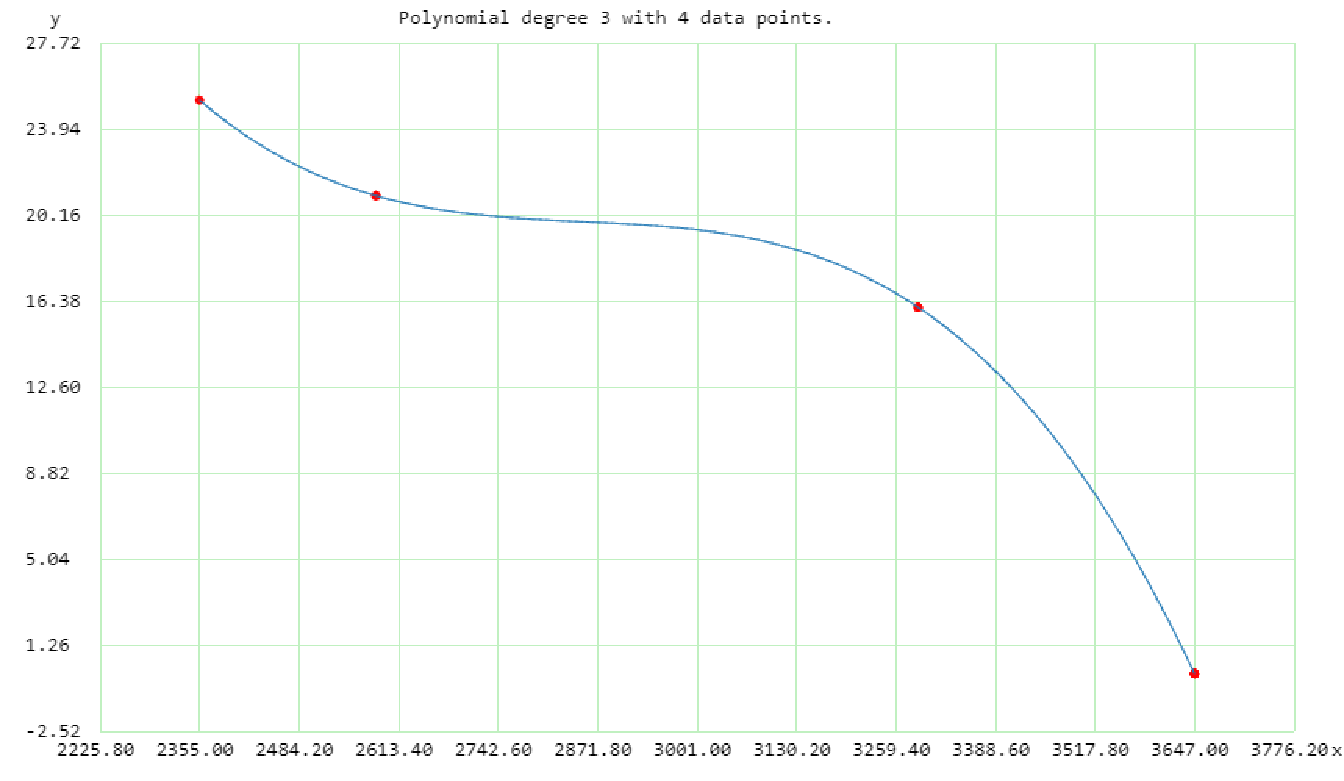
\includegraphics[width=\textwidth]{../images/regression}
    \caption{}
    \label{fig:regression}
\end{figure}


%% Anmerkung: Nur wichtige Implementierungsdetails sollen hier erklärt werden.
%% Code-Beispiele (snippets) können hier aufgelistet werden, um der Erklärung zu dienen.
%% Welche Patterns haben Sie für Ihre Implementierung benutzt.
%% Anmerkung: Bitte KEINE ganze Programme hierhin kopieren!
